\begin{frame}{意味のある「統計」期間について}{検証}
  \lead{実在するのは 1〜2 か月スケールの季節変化}
  \begin{columns}[T]
    \begin{column}{0.44\textwidth}
      \sub{1 年を $K$ 個の正弦波で表す（調和回帰）}
      \vskip -4mm
      {\small
      \begin{align*}
        \hat{\mathbf y}(d) = \mathbf a_0 + \sum_{j=1}^{K}\Bigl[&\mathbf a_j \cos\bigl(\tfrac{2\pi j d}{365}\bigr) \\[-1mm]
          &+ \mathbf b_j \sin\bigl(\tfrac{2\pi j d}{365}\bigr)\Bigr]
      \end{align*}}
      \vskip -3.5mm
      \begin{itemize}\itemsep 0.3mm
        \item 分解能 $\tau(K) = 365 / (2K)$ 日
        \item 誤差は \kw{$K = 5$--$6$} で頭打ち：$\tau \approx 30$--$36$ 日
        \item 半月ビンはこれを表現する単位
      \end{itemize}
    \end{column}
    \begin{column}{0.54\textwidth}
      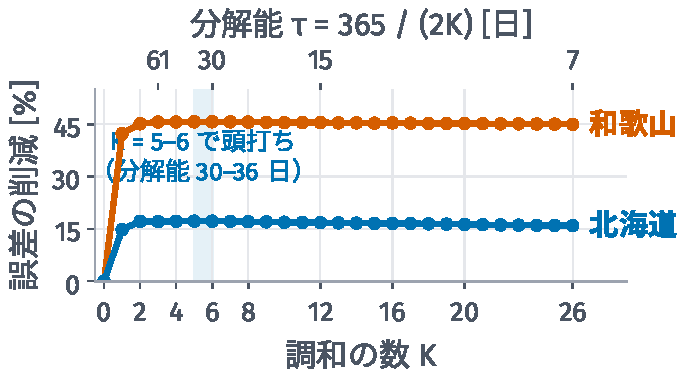
\includegraphics[width=\linewidth,height=124pt,keepaspectratio]{S_harmonic_overlay.pdf}
    \end{column}
  \end{columns}
  \srcline{1 年抜き交差検証、落下位置のベクトル RMSE}
\end{frame}
